\documentclass[12pt,a4paper]{article}
\usepackage[utf8]{inputenc}
\usepackage[T1]{fontenc}
\usepackage[serbian]{babel}
\usepackage{amsmath}
\usepackage{graphicx}
\usepackage{listings}
\usepackage{xcolor}

% Podešavanje izgleda koda u dokumentu
\definecolor{codegreen}{rgb}{0,0.6,0}
\definecolor{codegray}{rgb}{0.5,0.5,0.5}
\definecolor{codepurple}{rgb}{0.58,0,0.82}
\lstset{
	commentstyle=\color{codegreen},
	keywordstyle=\color{magenta},
	numberstyle=\tiny\color{codegray},
	stringstyle=\color{codepurple},
	basicstyle=\ttfamily\small,
	breaklines=true,
	captionpos=b,
	numbers=left,
	showstringspaces=false
}

\begin{document}
	
	\title{Predviđanje zagađenja vazduha (PM2.5 čestica) korištenjem mašinskog učenja}
	\author{Sasa Lakic RA220-2023}
	\maketitle
	
	\section{Implementacija programa}
	
	U ovom poglavlju opisan je proces učitavanja i inicijalne obrade podataka korišćenjem biblioteke \texttt{pandas} u jeziku Python.
	
	\subsection{Učitavanje i formatiranje vremenskih serija}
	
	Prvi korak u svakoj analizi vremenskih serija je pravilno rukovanje datumima. U nastavku je prikazana funkcija za učitavanje podataka:
	
	\begin{lstlisting}[language=Python, caption=Funkcija za učitavanje podataka]
		def load_air_quality_data(file_path):
		df = pd.read_csv(file_path)
		
		# Spajanje kolona u jedinstven datum
		df['date'] = pd.to_datetime(df[['year', 'month', 'day', 'hour']])
		df.set_index('date', inplace=True)
		
		# Selektovanje relevantnih kolona
		relevant_cols = ['PM2.5', 'TEMP', 'PRES', 'DEWP', 'RAIN', 'WSPM']
		df = df[relevant_cols]
		
		return df
	\end{lstlisting}
	
	\subsubsection{Obrazloženje postupka učitavanja}
	
	Korišćenje funkcije \texttt{pd.read\_csv} omogućava efikasno prebacivanje podataka iz tekstualnog formata u \texttt{DataFrame} strukturu koja je optimizovana za rad sa velikim količinama podataka. Ključni koraci u ovoj fazi su:
	
	\begin{itemize}
		\item \textbf{Konverzija u \texttt{datetime}:} Funkcija \texttt{pd.to\_datetime} spaja odvojene kolone (godina, mjesec, dan, sat) u jedinstven vremenski objekat. Ovo je neophodno jer algoritmi poput LSTM-a i Prophet-a moraju prepoznati hronološki redoslijed i cikličnost (npr. prelaz sa 23:00 na 00:00 narednog dana).
		\item \textbf{Postavljanje indeksa (\texttt{set\_index}):} Pretvaranjem kolone \texttt{date} u indeks, podaci se transformišu iz obične tabele u \textbf{vremensku seriju (Time Series)}. Ovo drastično olakšava kasnije operacije poput interpolacije nedostajućih vrijednosti i crtanja grafika, jer \texttt{pandas} tada automatski prepoznaje vremensku distancu između uzoraka.
	\end{itemize}
	
	\subsection{Pretprocesiranje i rješavanje problema nedostajućih vrijednosti}
	
	Sirovi podaci često sadrže nedostajuće vrijednosti (\textit{NaN}) koje mogu uzrokovati greške pri treniranju modela. Umjesto prostog brisanja redova, što bi narušilo kontinuitet vremenske serije, primijenjena je dvo-fazna strategija imputacije unutar funkcije \texttt{preprocess\_missing\_values}.
	
	\begin{lstlisting}[language=Python, caption=Metode za popunjavanje rupa u podacima]
		def preprocess_missing_values(df):
		# 1. Linearna interpolacija za kratke prekide
		df['PM2.5'] = df['PM2.5'].interpolate(method='linear', limit=2)
		
		# Privremene kolone za sezonsku analizu
		df['month'] = df.index.month
		df['hour'] = df.index.hour
		
		# 2. Imputacija na osnovu istorijskog prosjeka za dati sat i mjesec
		df['PM2.5'] = df['PM2.5'].fillna(
		df.groupby(['month', 'hour'])['PM2.5'].transform('mean')
		)
		
		df.drop(['month', 'hour'], axis=1, inplace=True)
		return df
	\end{lstlisting}
	
	\subsubsection{Obrazloženje strategije čišćenja}
	
	\begin{itemize}
		\item \textbf{Linearna interpolacija (\texttt{limit=2}):} Ova metoda se koristi za popunjavanje kratkih prekida (1 do 2 uzastopna sata). Pretpostavka je da se koncentracija PM2.5 čestica ne mijenja trenutno, već postepeno, pa je srednja vrijednost između dva susjedna sata logična aproksimacija.
		\item \textbf{Sezonska imputacija (\texttt{groupby}):} Za duže periode nedostatka podataka, koristi se prosjek za taj specifični sat u tom mjesecu. Na primjer, ako nedostaje podatak za 14:00h u januaru, sistem izračunava prosjek svih dostupnih mjerenja u 14:00h tokom svih januara u setu podataka. Time se čuva dnevni i sezonski profil zagađenja koji je ključan za rad Prophet modela.
		\item \textbf{Očuvanje dimenzionalnosti:} Na kraju funkcije, ukupan broj uzoraka ostaje nepromijenjen (35,064), što potvrđuje da nismo gubili informacije brisanjem redova.
	\end{itemize}
	
	\section{Eksplorativna analiza podataka (EDA)}
	
	Prije implementacije prediktivnih modela, izvršena je analiza korelacije i dekompozicija vremenske serije kako bi se identifikovali ključni faktori uticaja i sezonski obrasci.
	
	\subsection{Analiza korelacije meteoroloških faktora}
	
	Funkcija \texttt{run\_eda\_correlation} generiše matricu korelacije koja prikazuje linearnu povezanost između koncentracije PM2.5 čestica i atmosferskih prilika.
	
	\begin{lstlisting}[language=Python, caption=Vizuelizacija korelacije pomoću toplotne mape]
		def run_eda_correlation(df):
		plt.figure(figsize=(10,8))
		corr_matrix = df.corr()
		sb.heatmap(corr_matrix, annot=True, cmap='coolwarm', fmt=".2f")
		plt.title("Korelacija PM2.5 čestica sa meteorološkim faktorima")
		plt.show()
	\end{lstlisting}
	
	\subsubsection{Interpretacija rezultata korelacije}
	Na osnovu generisane toplotne mape (\textit{heatmap}), uočene su ključne zavisnosti:
	\begin{itemize}
		\item \textbf{Negativna korelacija sa brzinom vjetra (WSPM):} Jači vjetar doprinosi disperziji čestica, čime se smanjuje njihova koncentracija u vazduhu.
		\item \textbf{Korelacija sa temperaturom (TEMP):} Niže temperature su često povezane sa povećanim zagađenjem uslijed fenomena temperaturne inverzije i povećane potrošnje energenata za grijanje.
	\end{itemize}
	
	\begin{figure}[h!]
		\centering
		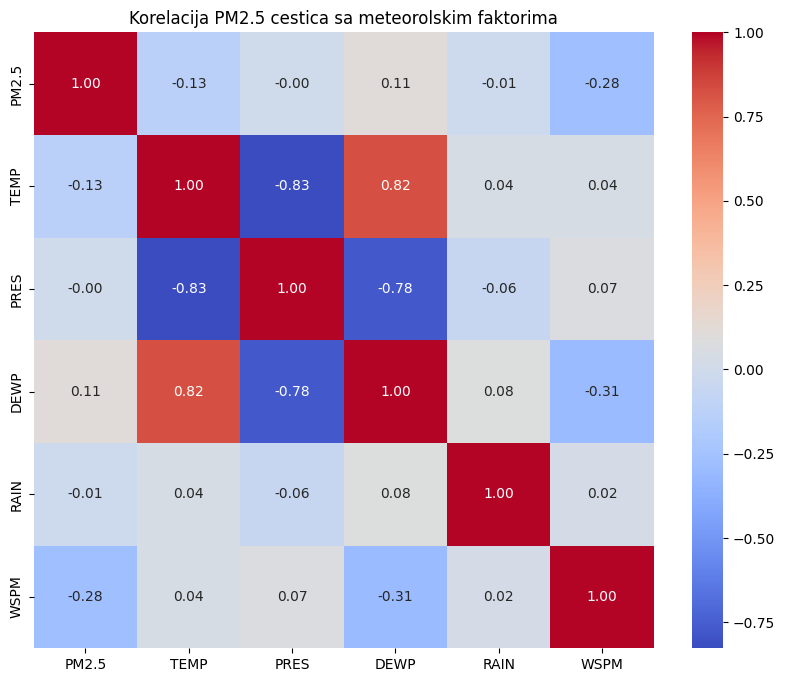
\includegraphics[width=0.8\textwidth]{eda.png}
		\caption{Matrica korelacije PM2.5 čestica i meteoroloških parametara}
		\label{fig:eda_heatmap}
	\end{figure}

	
	\subsection{STL Dekompozicija}
	
	Za dublje razumijevanje strukture vremenske serije korišćena je \textbf{STL dekompozicija} (\textit{Seasonal-Trend decomposition using LOESS}).
	
	\begin{lstlisting}[language=Python, caption=Dekompozicija vremenske serije]
		def run_stl_decomposition(df):
		subset = df['PM2.5'].tail(1000)
		# period=24 predstavlja dnevni ciklus (24 sata)
		res = STL(subset, period=24).fit()
		fig = res.plot()
		plt.suptitle('STL Dekompozicija: Trend, Sezonalnost i Reziduali')
		plt.show()
	\end{lstlisting}
	
	\begin{figure}[h!]
		\centering
		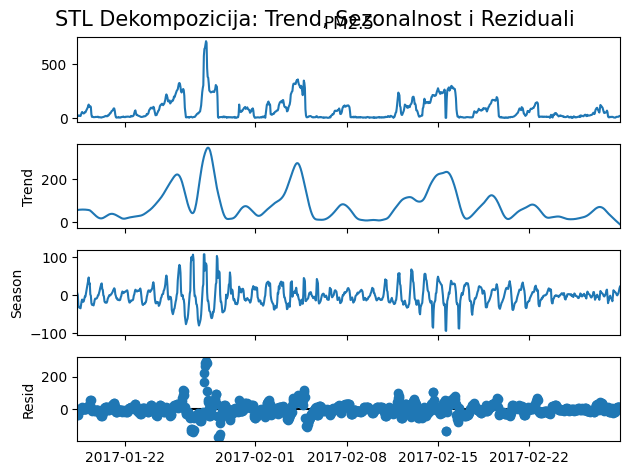
\includegraphics[width=0.9\textwidth]{stl.png}
		\caption{STL dekompozicija vremenske serije PM2.5 (Trend, Sezonalnost i Reziduali)}
		\label{fig:stl_plot}
	\end{figure}
	
	\subsubsection{Analiza komponenti dekompozicije}
	
	Na osnovu grafika prikazanog na Slici \ref{fig:stl_plot}, možemo identifikovati tri ključna elementa serije:
	\begin{itemize}
		\item \textbf{Trend:} Prikazuje dugoročno kretanje nivoa zagađenja, očišćeno od dnevnih fluktuacija.
		\item \textbf{Seasonal (Sezonalnost):} Jasno su vidljivi pravilni oscilatorni kretaji sa periodom od 24 sata, što potvrđuje snažan uticaj dnevnih ljudskih aktivnosti i meteoroloških ciklusa na koncentraciju čestica.
		\item \textbf{Resid (Reziduali):} Predstavljaju ostatak varijanse koji se ne može objasniti trendom niti sezonalnošću (npr. nagle promjene vremena ili incidentna zagađenja).
	\end{itemize}
	
	\section{ARIMA Model (Benchmark)}
	
	Kao bazni (\textit{benchmark}) model za predviđanje koncentracije PM2.5 čestica odabran je \textbf{ARIMA} model. Njegova uloga je da pruži osnovnu metriku preciznosti zasnovanu na čisto statističkim metodama analize vremenskih serija.
	
	\begin{lstlisting}[language=Python, caption=Implementacija ARIMA modela]
		def run_arima_model(df):
		# Podjela na trening i test (zadnjih 6 mjeseci za test)
		test_size = 4320 
		train = df['PM2.5'].iloc[:-test_size]
		test = df['PM2.5'].iloc[-test_size:]
		
		# Konfiguracija modela: (p, d, q) = (1, 1, 1)
		model = ARIMA(train, order=(1, 1, 1))
		
		# Optimizacija brzine izvrsavanja pomocu 'innovations_mle'
		model_fit = model.fit(method='innovations_mle') 
		
		# Predvidjanje naredna 24 sata
		forecast = model_fit.forecast(steps=24)
	\end{lstlisting}
	
	\subsection{Parametri i optimizacija}
	
	U modelu je korišćen \textbf{order=(1, 1, 1)}, što podrazumijeva:
	\begin{itemize}
		\item \textbf{p = 1 (AutoRegressive):} Model uzima u obzir vrijednost iz prethodnog sata.
		\item \textbf{d = 1 (Integrated):} Podaci se diferenciraju jednom kako bi se postigla stacionarnost (stabilizacija srednje vrijednosti).
		\item \textbf{q = 1 (Moving Average):} Model koristi grešku iz prethodnog koraka kako bi ispravio trenutnu predikciju.
	\end{itemize}
	
	Posebno važno za performanse na prenosnim računarima je korišćenje metode \texttt{innovations\_mle}, koja omogućava brže pronalaženje parametara modela bez gubitka značajne preciznosti.
	
	\subsection{Rezultati i evaluacija}
	
	Evaluacija modela izvršena je na prvih 24 sata testnog skupa podataka. Dobijeni rezultati su:
	\begin{itemize}
		\item \textbf{RMSE (Root Mean Squared Error):} 3.87
		\item \textbf{MAE (Mean Absolute Error):} 3.05
	\end{itemize}
	
	\begin{figure}[h!]
		\centering
		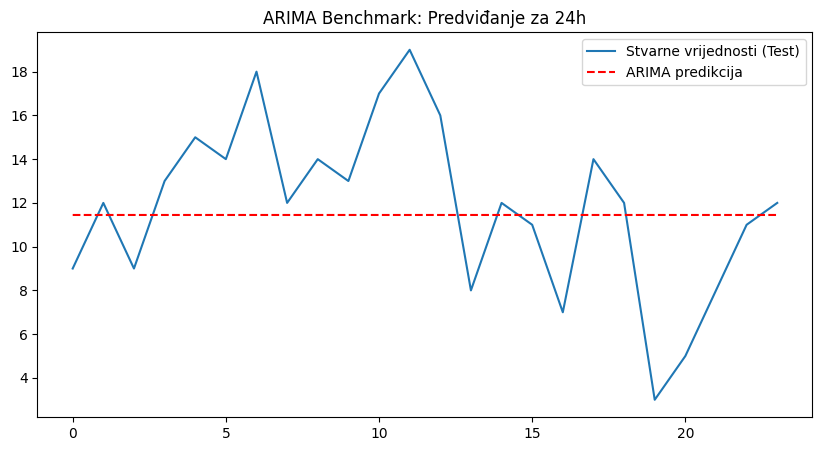
\includegraphics[width=0.85\textwidth]{arima.png}
		\caption{Poređenje stvarnih vrijednosti i ARIMA predikcije za period od 24h}
		\label{fig:arima_plot}
	\end{figure}
	
	Kao što se vidi na Slici \ref{fig:arima_plot}, ARIMA model teži ka "usrednjavanju" predikcije. Iako su greške RMSE i MAE relativno niske, model ne uspijeva u potpunosti da isprati nagle promjene (šiljke) u zagađenju, što je očekivano za linearne statističke modele.
	
	\section{Facebook Prophet Model}
	
	Za razliku od klasičnih statističkih modela, \textbf{Prophet} tretira predviđanje vremenskih serija kao problem prilagođavanja krive (\textit{curve fitting}), uzimajući u obzir praznike i ciklične komponente na više nivoa.
	
	\begin{lstlisting}[language=Python, caption=Implementacija Prophet modela]
		def run_prophet_model(df):
		# Prophet zahtijeva kolone ds (datum) i y (vrijednost)
		df_prophet = df.reset_index()[['date', 'PM2.5']]
		df_prophet.columns = ['ds', 'y']
		df_prophet['ds'] = df_prophet['ds'].dt.tz_localize(None)
		
		# Definisanje modela sa visestrukom sezonalnoscu
		model = Prophet(
		daily_seasonality=True, 
		weekly_seasonality=True, 
		yearly_seasonality=True
		)
		model.fit(train)
		
		# Generisanje buduceg vremenskog okvira za 24h
		future = model.make_future_dataframe(periods=24, freq='H')
		forecast = model.predict(future)
	\end{lstlisting}
	
	\subsection{Rezultati i analiza Prophet modela}
	
	Evaluacija modela na testnom skupu dala je sljedeće rezultate:
	\begin{itemize}
		\item \textbf{RMSE:} 24.88
		\item \textbf{MAE:} 23.80
	\end{itemize}
	
	\begin{figure}[h!]
		\centering
		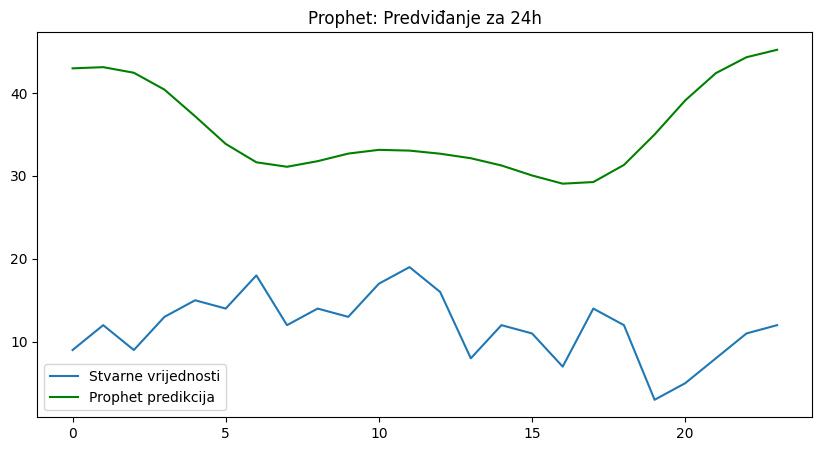
\includegraphics[width=0.85\textwidth]{prophet.png}
		\caption{Predviđanje koncentracije PM2.5 pomoću Prophet modela za period od 24h}
		\label{fig:prophet_plot}
	\end{figure}
	
	\subsubsection{Interpretacija lošijih metričkih rezultata}
	
	Zanimljivo je uočiti da su RMSE i MAE kod Prophet modela značajno viši nego kod ARIME. Razlozi za ovo leže u samoj prirodi modela:
	\begin{itemize}
		\item \textbf{Preveliko oslanjanje na sezonalnost:} Prophet pokušava da nametne "idealan" dnevni i sedmični profil. Ako se u testnom periodu desio nagli skok zagađenja koji nije u skladu sa istorijskim prosjekom za taj sat, Prophet će ga potpuno ignorisati, dok će se ARIMA (koja gleda zadnji sat) brže prilagoditi.
		\item \textbf{Aditivni model:} Prophet najbolje radi na serijama koje imaju jasne trendove rasta kroz godine, dok je zagađenje vazduha veoma haotično i zavisi od trenutnih meteoroloških promjena koje ovaj model ne vidi direktno.
	\end{itemize}
	
\end{document}